\chapter{Partial Tracking\label{chap:partialtracking}}

In the previous chapter, we saw how to estimate parameters of sinusoids with
polynomial phase. While theoretically applicable to signals of arbitrary length,
for reasons of flexibility and efficiency, we usually estimate the local
parameters of the signal under a low order model and connect multiple
estimations to form a partial. We will call these local estimations ``analysis
points'' or ``parameter sets''.

This chapter presents an interpretation of the \textit{peak matching} procedure
of McAulay and Quatieri \cite{mcaulay1986speech}, a classical approach to discovering partials. Our
interpretation allows for the specification of an arbitrary cost function
measuring the plausibility that a set of analysis points form the path of a
partial. With this path interpretation, we were able to design a technique that finds the
optimal set of paths under a constraint on the number of paths. The chapter
concludes with an example of partial tracking on a synthetic signal.

Typically the DTSTFT is computed for a block of contiguous samples, called a
\textit{frame} and these frames are computed every $H$ samples, $H$ being the
\textit{hop-size}. We will denote the $M$ sets of parameters at local maxima in
frame $h$ as $\theta_0^{h}, \dotsc, \theta_{M-1}^{h}$ and the $N$ in frame $h+1$
as $\theta_0^{h+1}, \dotsc, \theta_{N-1}^{h+1}$ where $h$ and $h+1$ refer to
adjacent frames. We are interested in paths that extend across $K$ frames where
each path touches only one parameter set and each parameter set is either
exclusive to a single path or is not on a path.

%In Section~\ref{sec:mqfmfromphase} we discussed how to determine reasonable
%values for the coefficients of a cubic phase polynomial by using the frequency,
%phase and time difference of two local maxima in the DTSTFT. In this section we
%discuss possible ways of determining which local maxima are connected. This is
%referred to as \textit{peak matching} \cite{mcaulay1986speech}
%or \textit{partial tracking} \cite{smith1987parshl} \cite{depalle1993tracking}.

\section{A Greedy Method}

In this section, we present the McAulay-Quatieri method of peak matching. It is
conceptually simple and a set of short paths can be computed quickly, but
it can be sensitive to spurious peaks and is optimal only in the sense that
the set of paths computed contains the best path possible --- the quality of the
other paths may be compromised under this criterion.

In \cite[p.~748]{mcaulay1986speech} the peak matching algorithm is described in
a number of steps; we summarize them here in a way comparable with the linear
programming formulation to be presented in the sequel. In that paper, the
parameters are the instantaneous amplitude, phase and frequency and are indexed
by frequency as $\omega_0^{h}, \dotsc, \omega_{M-1}^{h}$ and $\omega_0^{h+1},
\dotsc, \omega_{N-1}^{h+1}$ but we will allow for arbitrary parameter sets.
Define a distance function $\mathcal{D} \left( \theta_{i},\theta_{j} \right)$
that computes the similarity between $K=2$ sets of parameters. We will now
consider a method that finds $L$ pairs of parameters that are closest.

We compute the cost matrix $\boldsymbol{C}$
\[
    \boldsymbol{C} = \theta^{h} \otimes_{\mathcal{D}} \theta^{h+1}
\]
so that the $i$th row and $j$th column contain $C_{i,j} = \mathcal{D} \left(
\theta_{i}^{h},\theta_{j}^{h+1} \right)$.  For each $l \in \left[0 \dotsc L-1
\right]$, find the indices $i_{l}$ and $j_{l}$ corresponding to the shortest
distance, then remove the $i_{l}$th row and $j_{l}$th column from consideration
and continue until $L$ pairs have been determined or the distances exceed some
threshold $\Delta$. This is summarized in Algorithm~\ref{alg:mq_peak_match}

\iftoggle{formfudge}{%
    \medskip
}

\begin{algorithm}[H]
    \KwIn{the cost matrix $\boldsymbol{C}$}
    \KwOut{$L$ pairs of indices $\Gamma_{i}$ and $\Gamma_{j}$}
    $\Gamma_{i} \leftarrow \varnothing$\;
    $\Gamma_{j} \leftarrow \varnothing$\;
    \For{$l \leftarrow 0$ to $L-1$}{
        $\D i_{l},j_{l}=\argmin_{i \in \left[ 0,\dotsc,M-1 \right] \setminus
        \Gamma_{i}, j \in \left[ 0,\dotsc,M-1 \right] \setminus \Gamma_{j}}
        C_{i,j}$\;
        \If{$ C_{i_{l},j_{l}} > \Delta$}{
            \KwRet{$\Gamma_{i},\Gamma_{j}$}
        }
        $\Gamma_{i} \leftarrow \Gamma{i} \cup i_{l}$\;
        $\Gamma_{j} \leftarrow \Gamma{i} \cup j_{l}$\;
    }
    \KwRet{$\Gamma_{i},\Gamma_{j}$}
    \caption{A generalized McAulay-Quatieri peak-matching algorithm.}%
    \label{alg:mq_peak_match}
\end{algorithm}

\iftoggle{formfudge}{%
    \newpage%
}

This is a greedy algorithm because on every iteration the smallest cost is
identified and its indices are removed from consideration. Perhaps choosing a
slightly higher cost in one iteration would allow smaller costs to be chosen in
successive iterations. This algorithm does not allow for that. In other terms,
the algorithm does not find a set of pairs that represent a globally minimal sum of
costs.
Another drawback of the algorithm is that it only works between two successive
frames. The cost function could be extended to consider $K$ frames ($K$
arbitrary) of parameter sets, constructing a $K$-dimensional tensor instead of a
matrix, but assuming equal numbers of parameter sets in all frames, the search
space would grow exponentially with $K$. Nevertheless, the method is simple to
implement, computationally negligible when $K$ is small, and works well with a
variety of signals encountered in audio \cite{mcaulay1986speech}
\cite{smith1987parshl}.

\section{An Optimal Method \label{sec:lppathsearch}}

There is a way to find a set of paths over multiple frames ($K > 2$) having the
lowest total cost if
we restrict the search to exactly $L$ paths. Instead of indexing parameters by
their frame number $h$, we make $h$ part of the parameter set so that it can be
used by the distance function $\mathcal{D}$. Assume that over $K$ frames there
are $M$ total parameter sets. In this context we will consider them as nodes in
a graph. We define the vector $\boldsymbol{c} \in \mathbb{R}^{M^2}$
where the entry $\boldsymbol{c}_{i + Mj} = \mathcal{D} \left( \theta_{i}, \theta_{j}
\right)$. If we have a set of connections $\Gamma_{i,j}$ we can calculate the
total cost of these connections by defining the vector
\[
    \boldsymbol{x}_{i + Mj} = \begin{cases}
        1 & \text{there is a connection between }i\text{ and }j\\
        0 & \text{otherwise}
    \end{cases}
\]
and then forming the inner product
\[
    c_{\text{total}}=\left\langle \boldsymbol{c},\boldsymbol{x} \right\rangle
\]
Note that a node cannot be connected to itself. The question is how to find
$\boldsymbol{x}^{\ast}$ so that $c_{\text{total}}$ is minimized. If no
constraints are placed on $\boldsymbol{x}$, the solution is trivial, but not
useful. How do we constrain $\boldsymbol{x}$ to give us a solution to the
partial tracking problem? Let us consider an example.

In Figure~\ref{plot:simple_graph} we have an example of a simple graph or
lattice. Such a graph represents a plausible partial tracking situation:
vertically aligned nodes are parameter sets estimated from the same analysis
frame and we would like to connect these parameter sets between frames. The
numbers are indices of nodes in the graph and the possible connections between
them are indicated by lines, or \textit{edges}. Imagine that we would like to
find the two shortest paths. We will now examine the resulting paths from two
algorithms using different criteria for shortness.

In Figure~\ref{plot:simple_graph_greedy_paths} we find the paths using an
algorithm similar to Algorithm~\ref{alg:mq_peak_match} but search instead over a
tensor of distances $C \in \mathbb{R}^{3 \times 4 \times 2}$ whose entry
$C_{i,j,h}$ represents the cost of travelling on the path connecting the $i$th
node in layer 0, the $j$th node in layer 1 and the $h$th node in layer 2. This
cost is the sum of the euclidean distances giving the lengths of the
connections. This is the greedy method of searching for the best paths whose
optimality criterion is to find the set of best paths containing the absolute
best path. We see in Figure~\ref{plot:simple_graph_greedy_paths} that the
absolute shortest path, $1 \rightarrow 4 \rightarrow 8$, is discovered, followed
by the second shortest path not using the nodes of the first path, $2
\rightarrow 5 \rightarrow 7$.

\begin{figure}[!t]
    \centering
    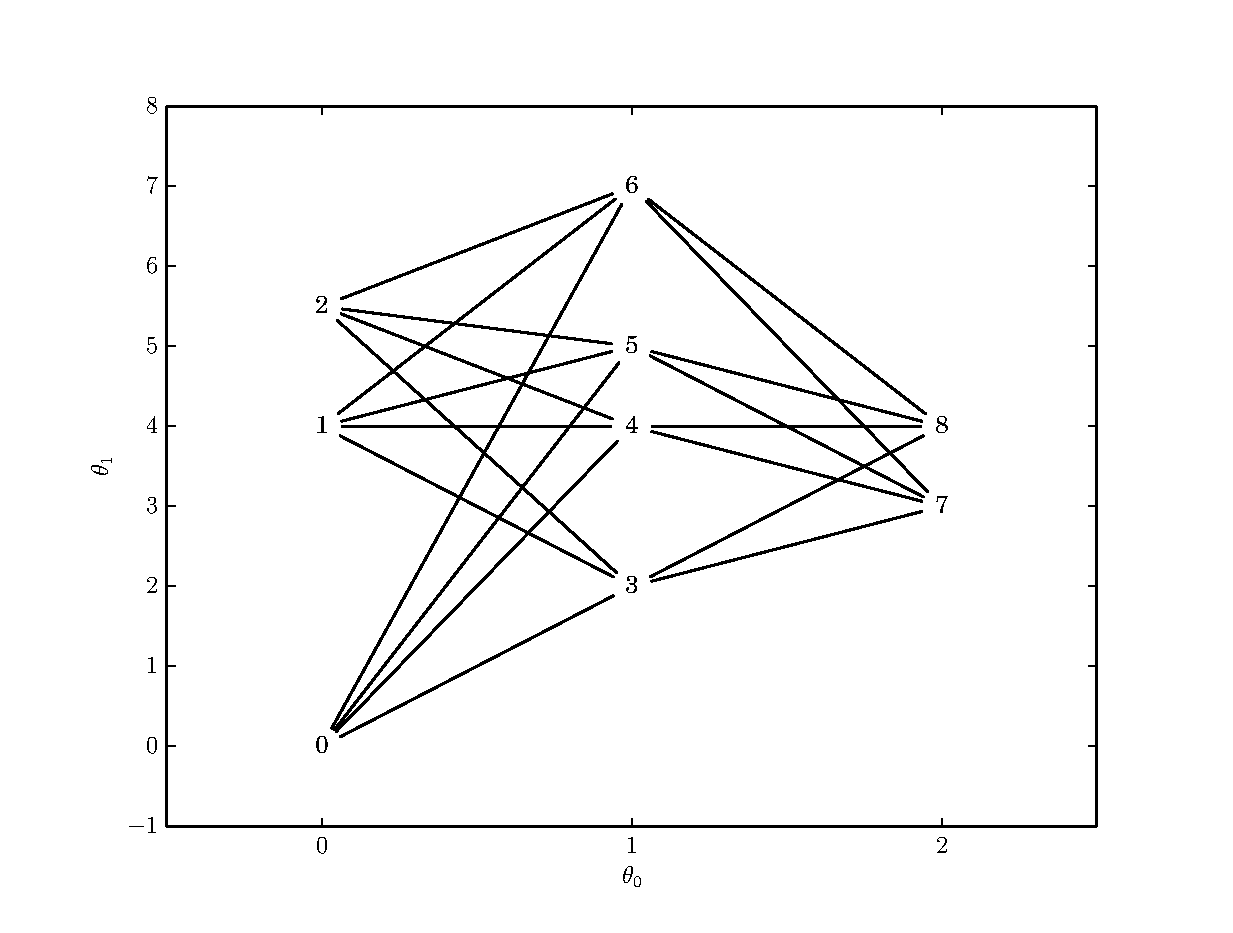
\includegraphics[width=\figwidthscale\textwidth]{plots/small_graph_ex.eps}
    \CaptionWithTitle{%
        \input{plots/small_graph_ex.txt}%
    }{\label{plot:simple_graph}}
\end{figure}

\begin{figure}[!t]
    \centering
    \includegraphics[width=\figwidthscale\textwidth]{plots/small_graph_ex_greedy_paths.eps}
    \CaptionWithTitle{%
        \input{plots/small_graph_ex_greedy_paths.txt}%
    }{\label{plot:simple_graph_greedy_paths}}
\end{figure}

\subsection{$L$ shortest paths via linear programming}

To find a set of paths minimizing the total cost, we instead search for total
solutions $\boldsymbol{x}$ that describe all paths in the graph. Assume for now
that we can guarantee that the entries of $\boldsymbol{x}$ will be either 0 or
1. To find a set of constraints for our search, we consider the structure of a
valid solution $\boldsymbol{x}^{\ast}$. To maintain that paths not overlap, a
valid solution's nodes are only allowed to have one edge entering ---
coming from a node in a previous frame --- and one edge leaving
--- going to a node in a successive frame. To translate this into a
constraint, consider the node $i$ and its possible $R_{i}$ successive connecting
nodes $j_{0} \dotsc j_{R_{i}-1}$. Define the vector\footnote{The superscript s
stands for ``successive''.}
\[
    a^{\text{s},i}_{i + Mj_{r}} = \begin{cases}
        1 & \forall j_{r} \in \left[ j_{0} \dotsc j_{R_{i}-1} \right] \\
        0 & \text{otherwise}
    \end{cases}
\]
As all the entries of $\boldsymbol{x}$ are either 0 or 1, we have
\[
    0 \leq \left\langle \boldsymbol{a}^{\text{s},i}, \boldsymbol{x} \right\rangle \leq 1
\]
so we can make this a constraint to ensure that a node has at most one path
leaving. Similarly, if we consider the node $j$ and its possible $R_{j}$ previous connecting
nodes $i_{0} \dotsc i_{R_{j}-1}$, the vector\footnote{The superscript p
stands for ``previous''.}
\[
    a^{\text{p},j}_{i_{r} + Mj} \begin{cases}
        1 & \forall i_{r} \in \left[ i_{0} \dotsc i_{R_{j}-1} \right] \\
        0 & \text{otherwise}
    \end{cases}
\]
constrains that node $j$ have only one path entering through the constraint
\[
    0 \leq \left\langle \boldsymbol{a}^{\text{p},j} , \boldsymbol{x} \right\rangle \leq 1
\]
A node on a path will also have an edge entering and an edge leaving. To
translate this into a constraint, we define a vector that counts the number of
edges entering a node and subtracts then the number of edges leaving a node. The
result should always be 0 for an equal number of edges entering and exiting a
node. If $r$ is the index of the node considered, the vector is simply
\footnote{The superscript b stands for ``balanced''.}
\[
    \boldsymbol{a}^{\text{b},r} = \boldsymbol{a}^{\text{p},r} -
    \boldsymbol{a}^{\text{s},r}
\]
and the constraint
\[
    \left\langle \boldsymbol{a}^{\text{b},r}, \boldsymbol{x} \right\rangle = 0
\]
Finally we want to constrain that there be only $L$ paths. We do this by
noticing that if this is true, there will be $L$ edges between frames $h$ and
$h+1$. We constrain the number of paths going from edges
$\Gamma_{h}$ in frame $h$ to $\Gamma_{h+1}$ by forming the vector
\footnote{The superscript c stands for ``connections''.}
\[
    \boldsymbol{a}^{\text{c},h} = \sum_{j \in \Gamma_{h}}
    \boldsymbol{a}^{\text{s},j}
\]
and asserting the constraint
\[
    \left\langle \boldsymbol{a}^{\text{c},h} , \boldsymbol{x} \right\rangle = L
\]
The length of $\boldsymbol{x}$ is $M^{2}$ so the total size of all the
constraints is not insignificant, but most entries in the constraint vectors will
be 0 and therefore the resulting constraint matrices very sparse, so sparse
linear algebra routines can be used in computations. Furthermore, the
$\boldsymbol{a}^{b}$ and $\boldsymbol{a}^{c}$ constraints are derived from
$\boldsymbol{a}^{p}$ and $\boldsymbol{a}^{s}$, so only the latter need to be
stored.

The complete \textit{linear program (LP)} solving the $L$ shortest paths problem is then
\begin{samepage}
\[
    \min_{\boldsymbol{x}} \left\langle \boldsymbol{c}, \boldsymbol{x} \right\rangle
\]
subject to
\[
    \boldsymbol{0} \leq
    \begin{bmatrix}
        \boldsymbol{A}_{\text{s}} \\
        \boldsymbol{A}_{\text{p}}
    \end{bmatrix} \boldsymbol{x}
    \leq \boldsymbol{1}
\]
\[
    \begin{bmatrix}
        \boldsymbol{A}_{\text{b}} \\
        \boldsymbol{A}_{\text{c}}
    \end{bmatrix}
    \boldsymbol{x}
    =
    \begin{bmatrix}
        \boldsymbol{0} \\
        L\boldsymbol{1}
    \end{bmatrix}
\]
\[
    \boldsymbol{0} \leq \boldsymbol{x} \leq \boldsymbol{1}
\]
\end{samepage}
where $\boldsymbol{A}_{\text{s}}$ is the matrix with
$\boldsymbol{a}^{\text{s},m}$ as its rows for $m \in [0 \dotsc M-1]$ and
$\boldsymbol{A}_{\text{p}}$ is the matrix with $\boldsymbol{a}^{\text{p},m}$ as
its rows, etc.

\begin{figure}[!t]
    \centering
    \includegraphics[width=\figwidthscale\textwidth]{plots/small_graph_ex_lp_paths.eps}
    \CaptionWithTitle{%
        \input{plots/small_graph_ex_lp_paths.txt}%
    }{\label{plot:simple_graph_lp_paths}}
\end{figure}

The solution of the two best paths using the LP formulation
is shown in Figure~\ref{plot:simple_graph_lp_paths} and a comparison of the
total costs is shown in Table~\ref{tab:greedy_lp_cost_compare}

\begin{table}
    \caption{\label{tab:greedy_lp_cost_compare} Comparison of total costs}
    \begin{center}
        \begin{tabular}{c c}
            Greedy & LP \\
            \hline
            \input{plots/small_graph_ex_greedy_cost.txt} &
            \input{plots/small_graph_ex_lp_cost.txt} \\
        \end{tabular}
    \end{center}
\end{table}

The LP formulation is inspired by a multiple object tracking algorithm for video
\cite{jiang2007linear}. A proof that the solution $\boldsymbol{x}^{\ast}$ will
have entries equal to either $0$ or $1$ can be found in
\cite[p.~167]{parker1988discrete}. The theoretical computational complexity of
the linear program is polynomial in the number of variables, see
\cite{karmarkar1984new} for a proof and the demonstration of a fast algorithm
for finding its solution. In practice, to extract paths from the solution, we do
not test equality with $0$ or $1$ but rather test if the solution vector's
values are greater than some threshold. This may mean that suboptimal solutions
may still be close enough. The tolerance of the solutions to suboptimality
should be investigated, as if they are tolerant, fewer iterations of a
barrier-based algorithm would be required to solve the problem. More information
on linear programming and optimization in general can be found in
\cite{boyd2004convex}.

\subsection{Complexity}

The LP formulation of the $L$-best paths problem gives results equivalent to the
solution to the $L$-best paths problem proposed in \cite{wolf1989finding}. The
complexity of our algorithm is different from that in this paper.  Assuming we
use the algorithm in \cite{karmarkar1984new} to solve the LP, our program has a
complexity of $O(M^{7}B^{2})$ where $M$ is the number of nodes (parameter sets)
and $B$ is the number of bits used to represent each number in the input. The
complexity of the algorithm by Wolf in \cite{wolf1989finding} is equivalent to
the Viterbi algorithm for finding the single best path through a trellis whose
$h$th frame has $\binom{N_{h}}{L}\binom{N_{h+1}}{L}L!$ connections where $N_{h}$
and $N_{h+1}$ are the number of nodes in two consecutive frames of the original
lattice. Therefore, assuming a constant number $N$ of nodes in each frame, its
complexity is $O((\binom{N}{L}^{2}L!)^{2}T)$. If there are few nodes in each
frame and a small number of paths are searched, Wolf's formulation is superior
as its complexity increases linearly with the number of frames in the lattice.
On the other hand, if each frame has a large number of nodes or many paths are
searched, the LP formulation is superior.  Informally we have found this to
agree with reality --- both algorithms were tried when producing the figures in
Section~\ref{sec:mq_lp_compare_chirp}.  Indeed the Wolf formulation took
prohibitively long to compute when many paths were desired, as did the LP when
many frames were considered.

It should be noted that in the special case that only 1 shortest path is
searched an algorithm exists that requires on the order of $N^{2}T$ calculations
\cite{rabiner1989tutorial} where $N$ is the number of nodes in each frame and
$T$ is the number of frames (assuming the same number of nodes in each frame):
this algorithm is known as the Viterbi algorithm \cite{forney1973viterbi}.

\section{Partial paths on an example signal\label{sec:mq_lp_compare_chirp}}

\begin{figure}[!t]
    %\centering
    \centering
    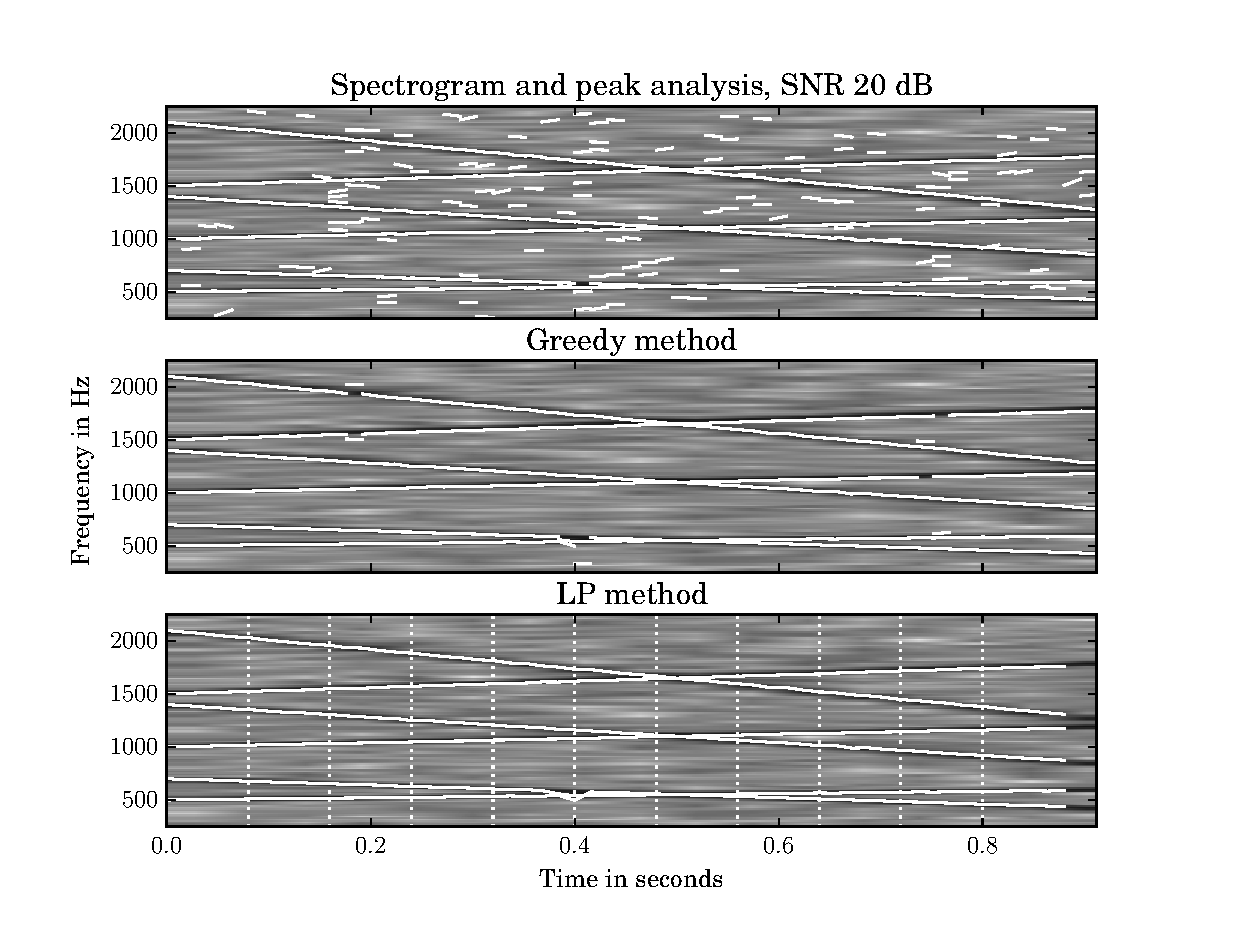
\includegraphics[width=\figwidthscale\textwidth]{plots/mq_lp_compare_chirp_20.eps}
    \CaptionWithTitle{%
        \input{plots/mq_lp_compare_chirp_20.txt}%
    }{ Line-segments representing the discovered partial paths.
    \label{plot:mq_lp_compare_chirp_20}}
\end{figure}
\begin{figure}[!t]
    %\centering
    \centering
    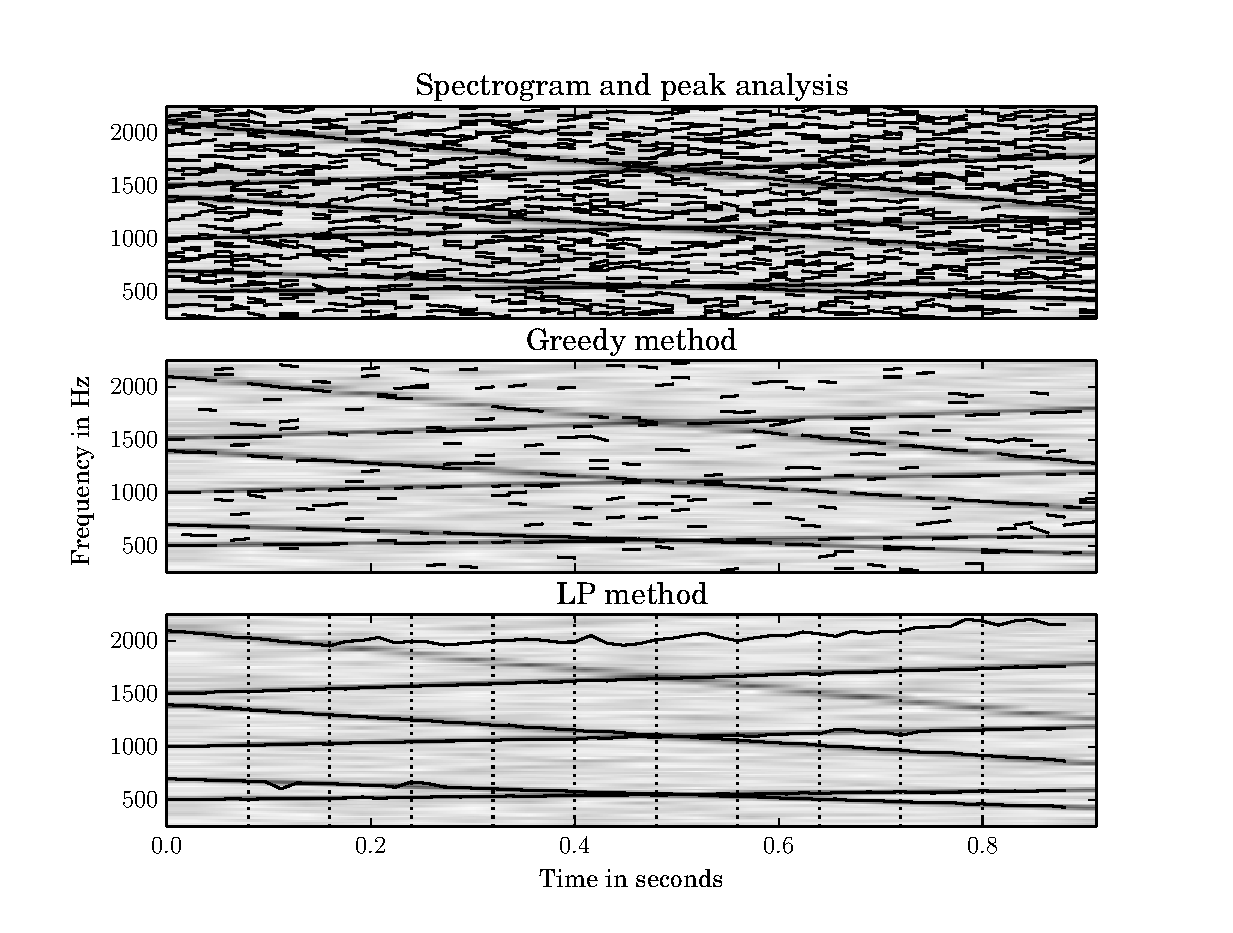
\includegraphics[width=\figwidthscale\textwidth]{plots/mq_lp_compare_chirp_15.eps}
    \CaptionWithTitle{%
        \input{plots/mq_lp_compare_chirp_15.txt}%
    }{ Line-segments representing the discovered partial paths.
    \label{plot:mq_lp_compare_chirp_15}}
\end{figure}
\begin{figure}[!t]
    %\centering
    \centering
    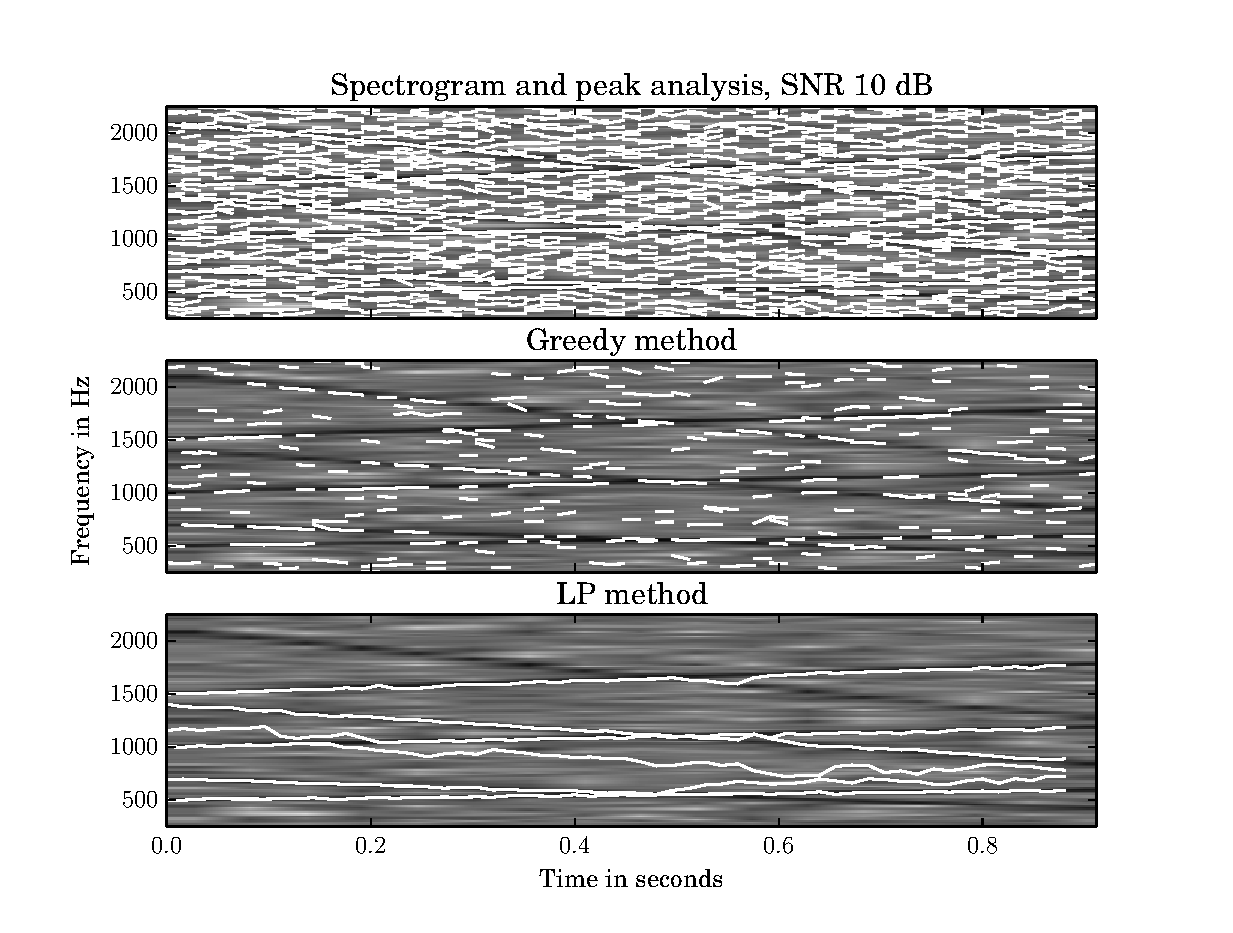
\includegraphics[width=\figwidthscale\textwidth]{plots/mq_lp_compare_chirp_10.eps}
    \CaptionWithTitle{%
        \input{plots/mq_lp_compare_chirp_10.txt}%
    }{ Line-segments representing the discovered partial paths.
    \label{plot:mq_lp_compare_chirp_10}}
\end{figure}

We compare the greedy and LP based methods for peak matching on a synthetic
signal. The signal is composed of $K=6$ chirps of constant amplitude, the $k$th
chirp $s$ at sample $n$ described by the equation
\[
    s_{k}(n) = \exp(j(\phi_{k} + \omega_{k}n +
    \frac{1}{2} \psi_{k} n^{2}))
\]
The parameters for the 6 chirps are presented in
Table~\ref{tab:ptrackexamplechirpparams}.
\begin{table}
    \caption{Parameters of $k$th chirp. $f_{0}$ and $f_{1}$ are the initial and
    final frequency of the chirp in Hz. \label{tab:ptrackexamplechirpparams}}
    \begin{center}
        \begin{tabular}{l c c c c c}
            $k$ & $\phi_{k}$ & $\omega_{k}$ & $\psi_{k}$ & $f_{0}$ & $f_{1}$ \\
            \hline
            \input{plots/mq_lp_compare_chirp_params.txt}
        \end{tabular}
    \end{center}
\end{table}

Two 1 second long signals are synthesized at a sampling rate of 16000 Hz, the
first with chirps 0--2, the second with chirps 3--5. We add
Gaussian distributed white noise at several SNR to evaluate the technique in the
presence of noise.

A spectrogram of each signal is computed with an analysis window length of 1024
samples and a hop-size $H$ of 256 samples. Local maxima are searched in 150 Hz
wide bands spaced 75 Hz apart. A local maximum is only accepted if its amplitude
is greater than -20 dB. At each local maximum the DDM is used to estimate the
local chirp parameters, the $i$th set of parameters in frame $h$ denoted
$\theta_{i}^{h} = \left\{ \phi_{i}^{h} , \omega_{i}^{h} , \psi_{i}^{h}
\right\}$. The results of the analyses of both signals are lumped together and
it is on this lumped data that we perform partial tracking.

We search for partial tracks using both the greedy and LP strategies. Both
algorithms use the distance metric $\mathcal{D}_{\text{pr.}}$ between two parameters sets:
\[
    \mathcal{D}_{\text{pr.}} \left( \theta_{i}^{h},
    \theta_{j}^{h+1} \right) = \left( \omega_{i}^{h} +
    \psi_{i}^{h} H - \omega_{j}^{h+1} \right)
\]
which is the error in predicting $j$th frequency in frame $h+1$ from the $i$th
parameters in frame $h$. For the greedy method, the search for partial paths is
restricted to one frame ahead like in \cite{mcaulay1986speech}. For the LP
method, to keep the computation time reasonable, we search over 6 frames for 6
best paths\footnote{The number of paths does not affect the computation time.}.
To maintain connected paths, the search on the next frames uses the end nodes of
the last search as starting points. For both methods, the search is restricted
to nodes between frequencies 250 to 2250 Hz.

Figures~\ref{plot:mq_lp_compare_chirp_10},~\ref{plot:mq_lp_compare_chirp_15}~and~\ref{plot:mq_lp_compare_chirp_20}
show discovered partial trajectories for signals with a SNR of 10, 15 and 20 dB
respectively. We can see that while the greedy method begins to perform poorly
at a SNR of 15dB, the LP method still gives plausible partial trajectories for
SNRs of 10 and 15 dB. At lower signal to noise ratios, the LP formulation gives
some paths that do not correspond to an underlying partial. These could be filtered
out by examining the cost of these paths and comparing them to the costs of the
others. Those that deviate from a mean cost more than a certain amount should be
rejected. This is the strategy used in Chapter~\ref{chap:decaysep} and
illustrated in Figure~\ref{plot:acgtra3xylofs4costlengththresh}. In any case,
the lower SNRs are relatively challenging for any partial tracking technique.

But why did the LP discover a path not present in the underlying signal? This is
due to the cost function, which finds a path with minimum prediction error in
using the frequency and frequency slope coefficients of one node to predict
another node's frequency coefficient. When there are many nodes in the original
analysis it is not surprising that some unexpected path exists.  An attribute of
these erroneous paths is that they are not smooth. To deter the algorithm from
finding such paths, regularization could be used like in
Section~\ref{sec:mqfmfromphase} that minimizes the integral of the squared
estimate of the path's second derivative. More on regularization in optimization
can be found in \cite[ch.~6.3]{boyd2004convex}.

\section{Conclusion}

In this chapter we reformulated the classical greedy algorithm of McAulay and
Quatieri and showed that it can be seen as a greedy algorithm for finding the $L$
shortest paths in a lattice. An algorithm was then proposed minimizing the sum
of the $L$ paths, using a linear programming approach. It was shown on synthetic
signals that the new approach finds plausible paths in lattices with a
large number of spurious nodes.

There are problems with the proposed approach. As discussed in
\ref{sec:lppathsearch}, ``jagged'' paths should be removed using regularization.
There are also situations where it is undesirable to have paths extend
throughout the entire lattice. Acoustic signals produced by striking media, such
as strings or bars, exhibit a spectrum where the upper partials decay more
quickly than the lower ones (e.g., see Figure~\ref{plot:acgtra3specgram}) --- it
would be desirable in these situations to have shorter paths for the upper
partials, those decaying more quickly. This could be addressed as in
\cite{depalle1993tracking} where the signal is divided into overlapping sequences of
frames and partial paths are connected between sequences.

The proposed algorithm, while faster than algorithms based on the Viterbi
algorithm, is still not fast. Assuming the same cost function
$\mathcal{D}_{\text{pr.}}$ as in Section~\ref{sec:mq_lp_compare_chirp} it would
be more efficient to consider narrow bands over which to search for paths when
analysing signals with little frequency modulation. However, as we will see in
Chapter~\ref{chap:amfmsep}, with different cost functions, the algorithm is
useful for solving general $L$ shortest paths problems outside of partial
tracking. 

% Problems:
% We assume paths spanning entire analysis are optimal

% Could also try and maximize smoothness of trajectories by adding second order
% differences as a cost.

%As a further test, we give the algorithms a hint by
%removing all spurious data-points from the first frame. We can see in
%Figures~\ref{plot:mq_lp_compare_chirp_hint15}~and~\ref{plot:mq_lp_compare_chirp_hint20}
%that this improves the results for the LP method.
